%!TEX root = project.tex

\chapter{System Design}
\section{Overview}
The purpose of this project was to create a multiplayer racing game, with the capability to be played on both desktop and VR headset and mobile. The game will have a log in system and will be handled by a C\# and Java with usernames and passwords saved on a Mongo database on a virtual machine.
\newline

Players will have the ability to either host or join a game in progress. This match making system will be handled by a mix of both C\# and Go programs. It will involve saving a list of players willing to host on a Redis database on a virtual machine and sending back the list to the game for player to join them.
\newline

The game will be a kart racing game, with desktop players using a kart while the VR players will be using a motorbike. Player on VR will be able to see the desktop player, and players on desktop will be able to see the VR players. Desktop player will also be able to see the VR players hand movements and gestures.
\newline

The game will have a procedural track created as the game starts. This track is created on the hosts machine and is shared with the players who have joined. Controls for the desktop will be:
W for forward, A for left, D for right, S for reverse and spacebar to jump and R to respawn.
VR controls will be A to jump and B to respawn.
\newline

Once the race is over, the player names and scores are sent to a scoreboard. These results are then sent to a Maria database running on the virtual machine and is handled by C\# and Python programs. The database will update the new results and a leader board is sent back to the host and displayed on screen.

\section{Log-in System}
When the user starts the program, they are presented with a login page. The user is prompted to enter a username and password to proceed. The username must be unique, having multiple users with the same username would cause confusion, and the password must be a minimum of eight characters long. If the user already has an account they simply enter their details and click login to proceed.
\newline 

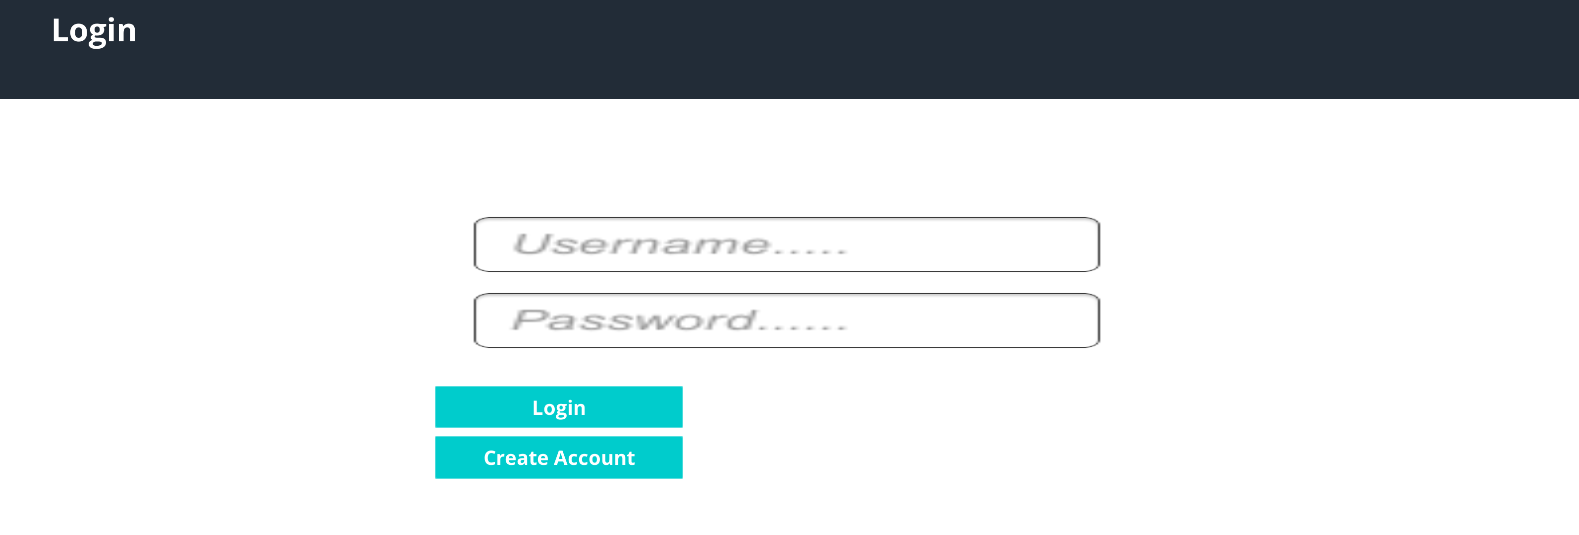
\includegraphics[width=1\columnwidth]{img/LoginActual.PNG}

 If the user is new to the game and does not have an account set up they must click create account and register as a user. Once the user is registered and logged in they get redirected to the match maker page to choose what they want to do next, host or join a game. 
\newline

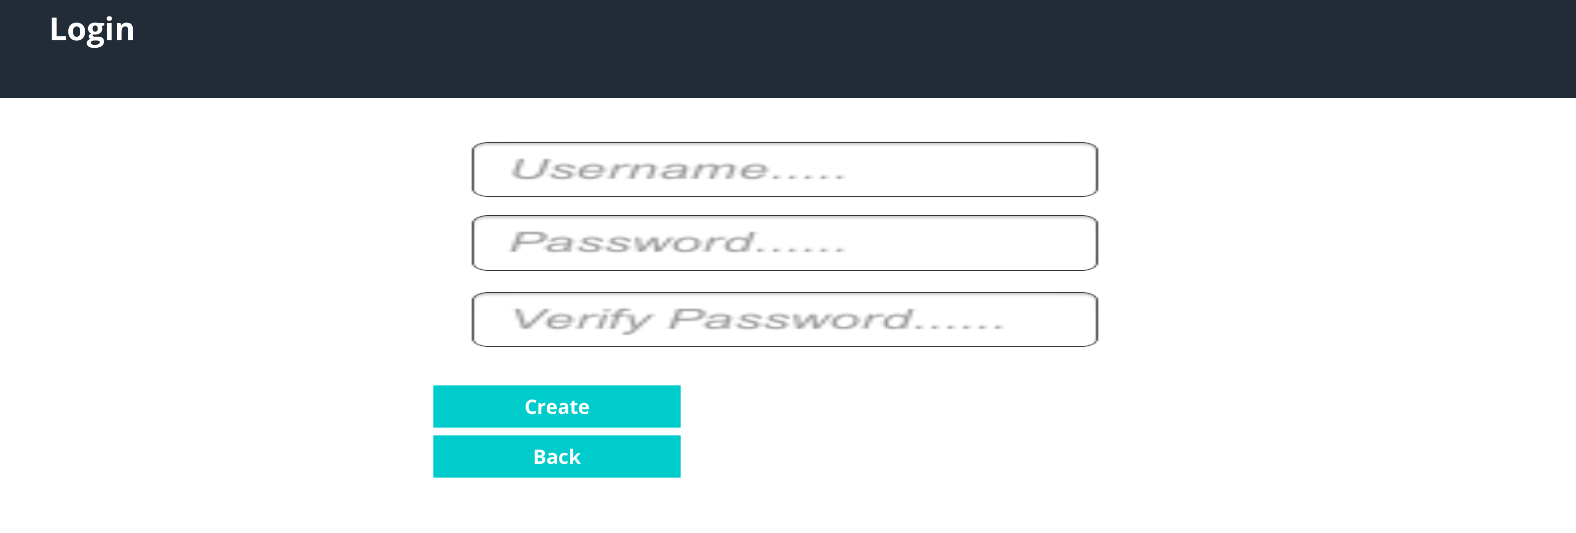
\includegraphics[width=1\columnwidth]{img/CreateAccountActual.PNG}

\section{Hosting a Game}
Once the user has logged in or created a new account, they are presented with the option to host or join an already hosted game. If the user wishes to host a game, they can press the host button. This will then take the users player name and IP Address and store them as a player object.
\newline

This object is then sent to the virtual machine and is received by a Go program, the object is then pushed into a struct. This struct is then sent to the Redis data base and stored until someone wants to join a game. The host is then sent to the game lobby to wait for other players to join. 
\newline

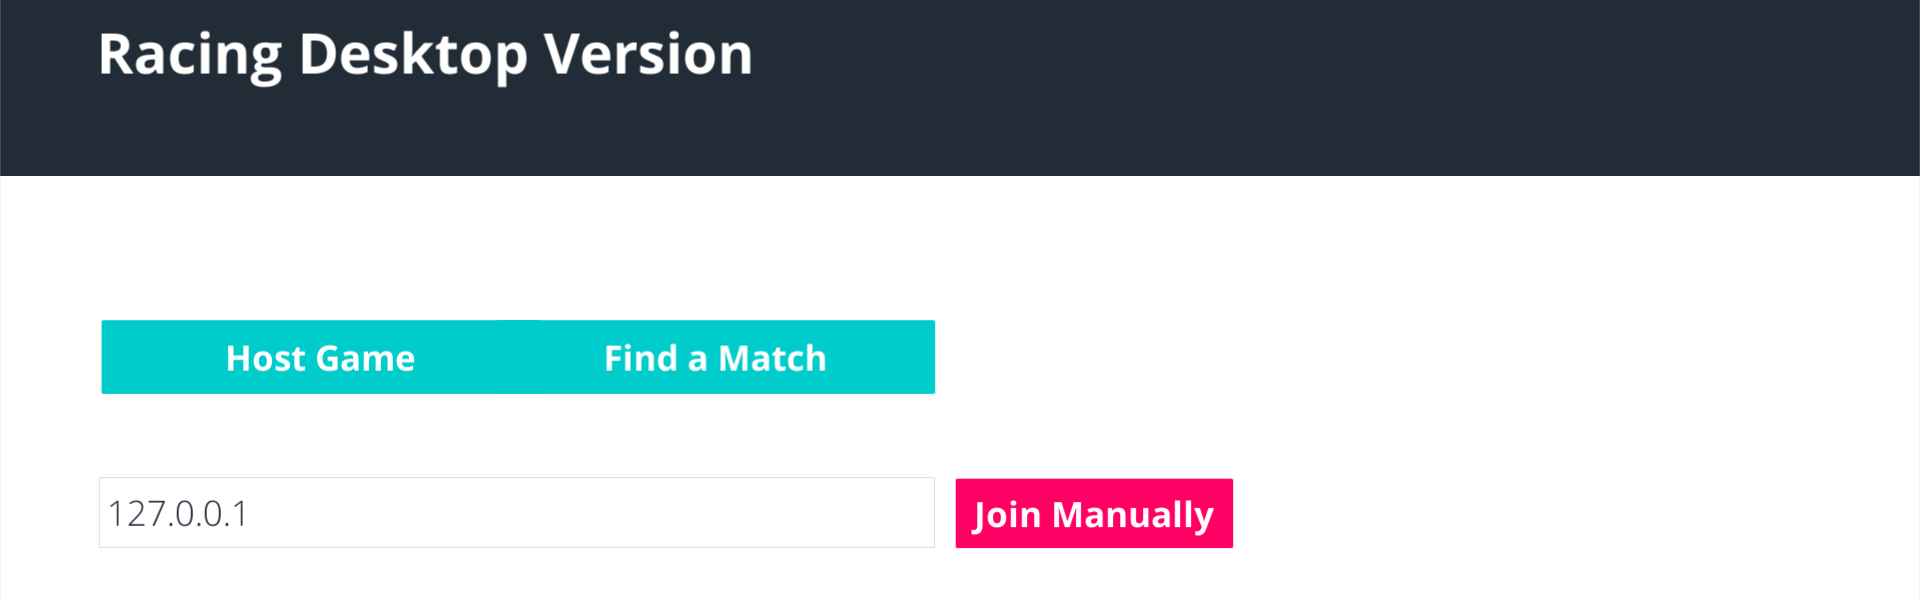
\includegraphics[width=1\columnwidth]{img/MatchFinder1Actual.PNG}

\section{Joining a game}
When the user clicks find a game. The program sends a request to the Redis database and gets back a list of games being hosted. The player can then select to join one the games that are displayed. When the user has joined the game they are brought to the lobby page.
\newline

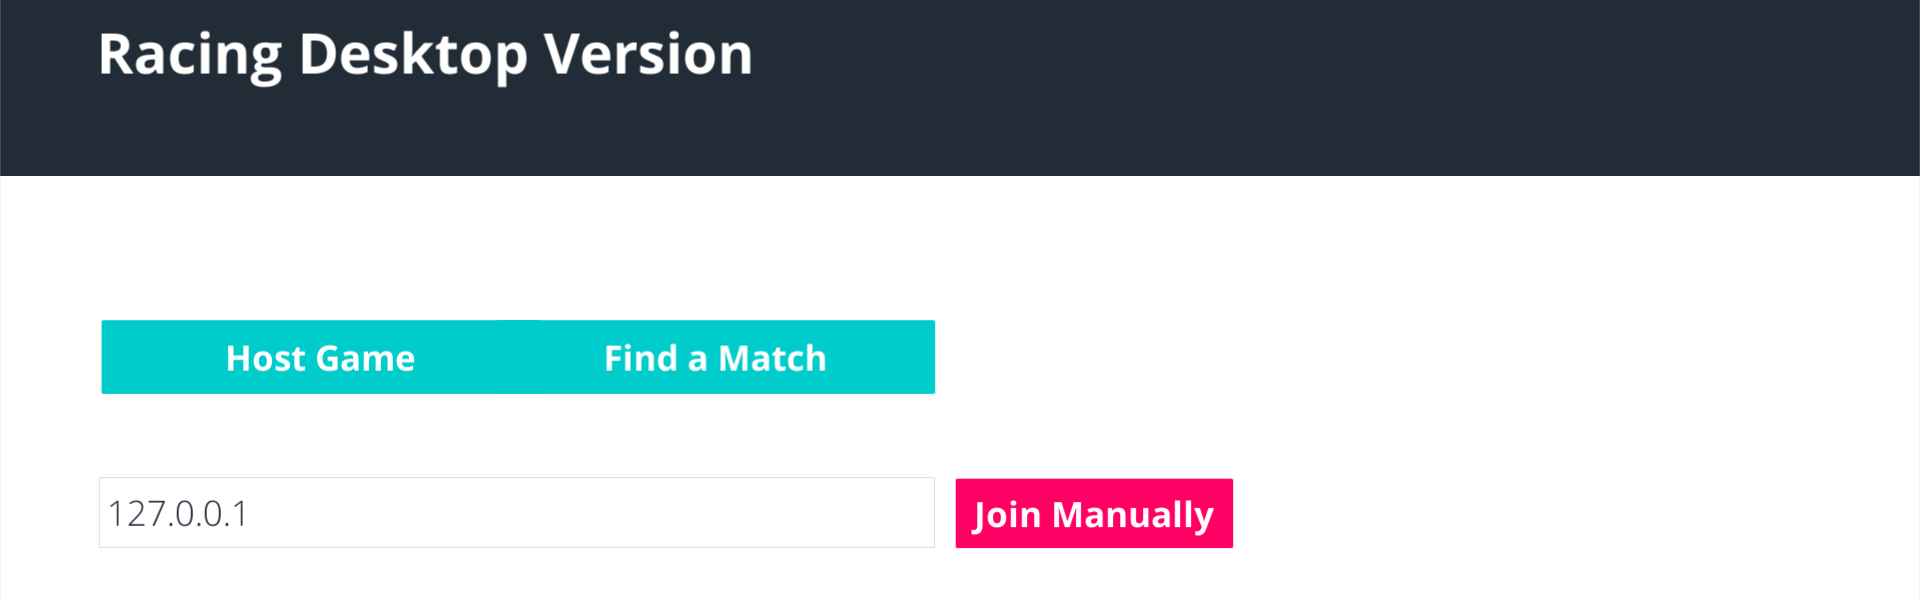
\includegraphics[width=1\columnwidth]{img/MatchFinder1Actual.PNG}

\section{In Game Lobby}
The host player is sent to the lobby immediately and then they wait for other players to join. As other players join the lobby there name is displayed on the screen. At anytime while in the lobby they can click join. When all players in the lobby click join they are presented with a counter that counts down from three. They are then sent to the race start. \newline

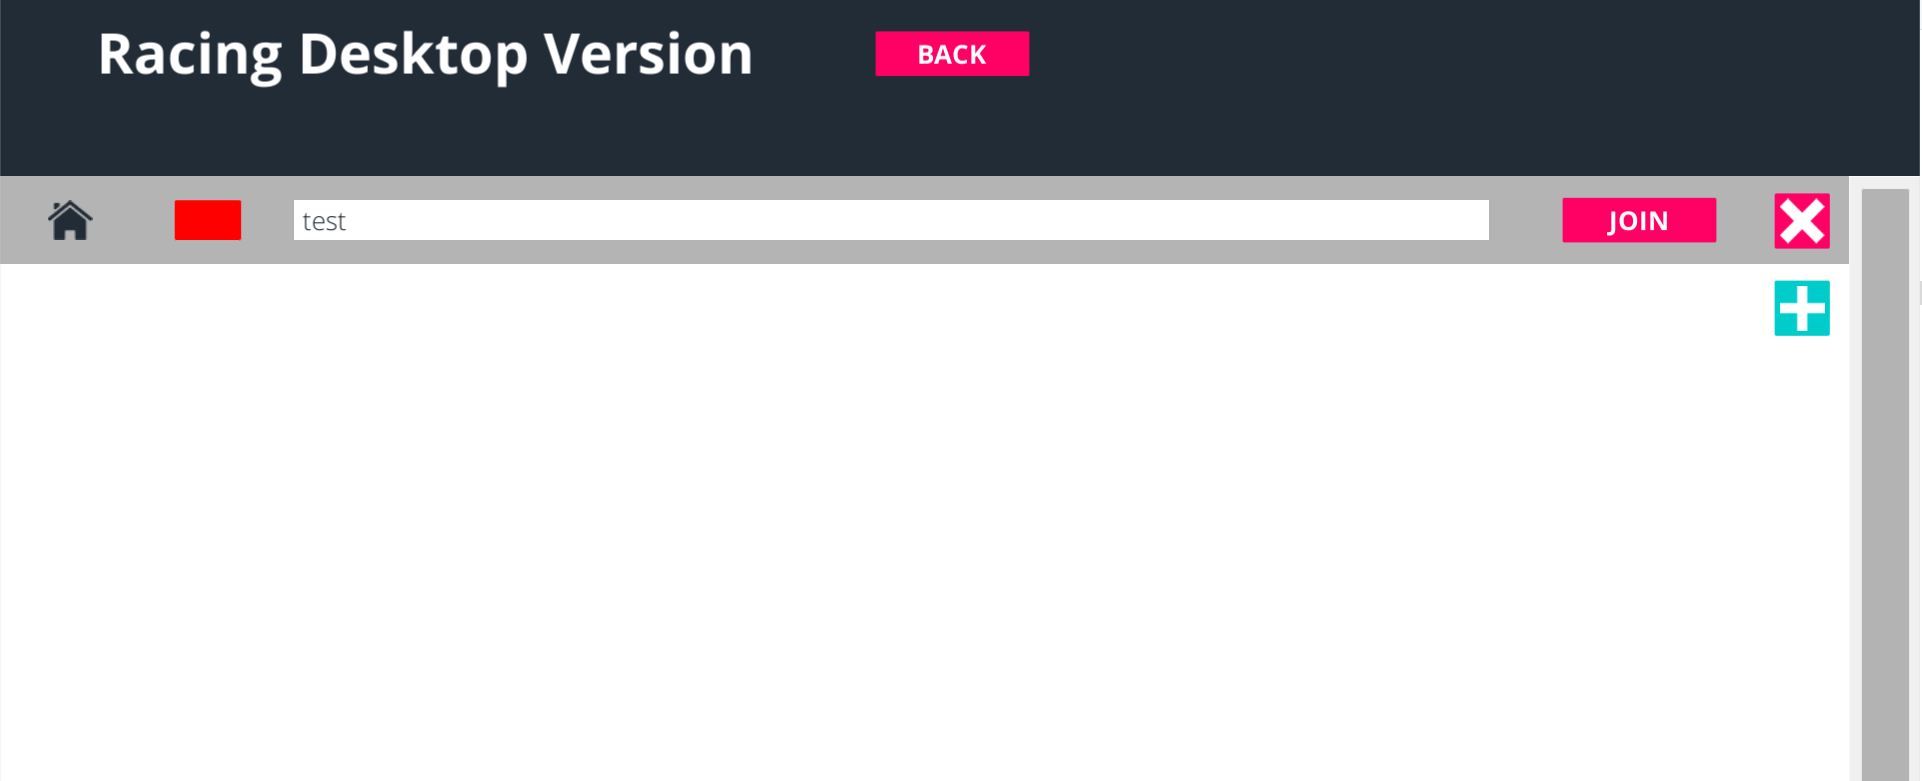
\includegraphics[width=1\columnwidth]{img/LobbyActual.PNG}

\section{The Game on Desktop}
The game on desktop consists of the player controlling a kart with the game character Morty (desktop only). The player lines up alongside his competitors to wait for the race to begin. Once the race starts the players race each other to the finish line on a procedural generated track that varies for each race.\newline

Desktop Player Controls:
\begin{itemize}
\item W moves the player forward.
\item A moves the player to the left.
\item S moves the player in reverse.
\item D moves the player to the right.
\item R re-spawns the player.
\item Space-bar allows the player to jump. 
\end{itemize}
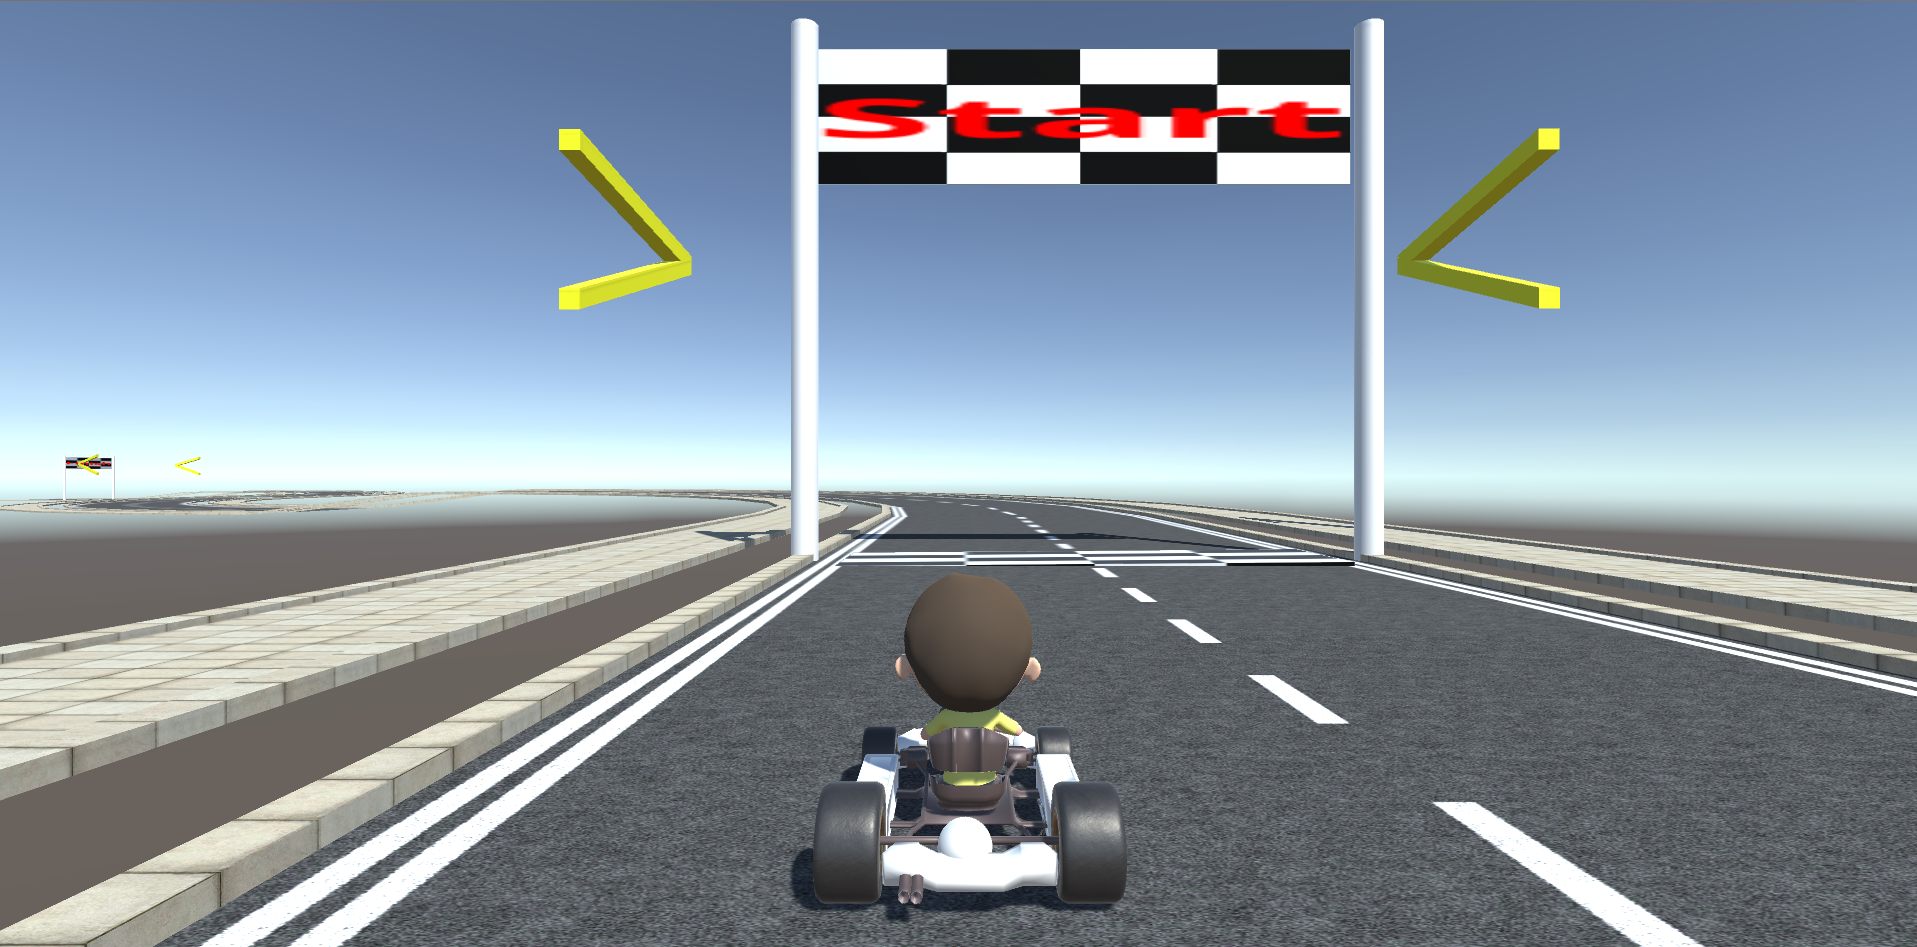
\includegraphics[width=1\columnwidth]{img/GameActual.PNG}

\section{The Game in Virtual Reality}

\textbf
The virtual reality section of the game is implemented differently from the desktop version of the game. In place of using a traditional monitor, the virtual reality devices use a head mounted display unit that utilises the full motion and direction of the users head, as if the person is actually in the game. With some of the virtual reality devices, players can use controllers that track the positions of the players hands. The players can use the buttons on the controllers to operate some functions of the game, such as jumping or grabbing an object.\newline

For our implementation of the game, we used the A button to jump, the B button to respawn. The two hat analog sticks pressed at the same time will re-center the camera of the players camera. We then imported some hands that are tracked by 3 sensors that are placed around the parameter of the players play space. the players hands move in real time with the player and can act just like real hands, given the right animations.\newline 

We were able to implement these features using the Oculus SDK. Some of the issues that had presented during the project were usually to do with the hardware rather than software. For instance the left earphone on the headset was damaged and had to be returned to Oculus which took two months for it to be returned.\newline

\section{Procedural Track}
A decision was made for the host to generate the race tracks in a procedural manner to keep consistency throughout the different platforms of the game. This would guarantee each player who joins a game would be racing on an identical track to everyone else who is playing either on desktop or VR. This also reduced the need to create multiple tracks, as the tracks that are generated are different for each race. This was a good decision on our behalf as the original plan was to create the race track on desktop and then recreate it in VR. This would have been a very time consuming and troublesome process.\newline

Originally we had mathematically generated this track, however a mistake was made that sometimes caused a bug where the track would generate a piece out of line on the track. So the approach was changed. Instead of mathematically calculating where each piece should appear, we created a set of track pieces, for example, one straight road piece and a left and right turn. Then some pieces that allow the track to descend or ascend. Each prefab for the track has two markers, one marker at the starting position. Then another marker at an ending position, which is the point where the next piece should join on to the current piece. So when the program creates the track, it slots the road pieces together like lego. Generate one piece at point 0.0, then randomly pick the next track piece and place its starting marker at the ending marker of the previous piece.\newline

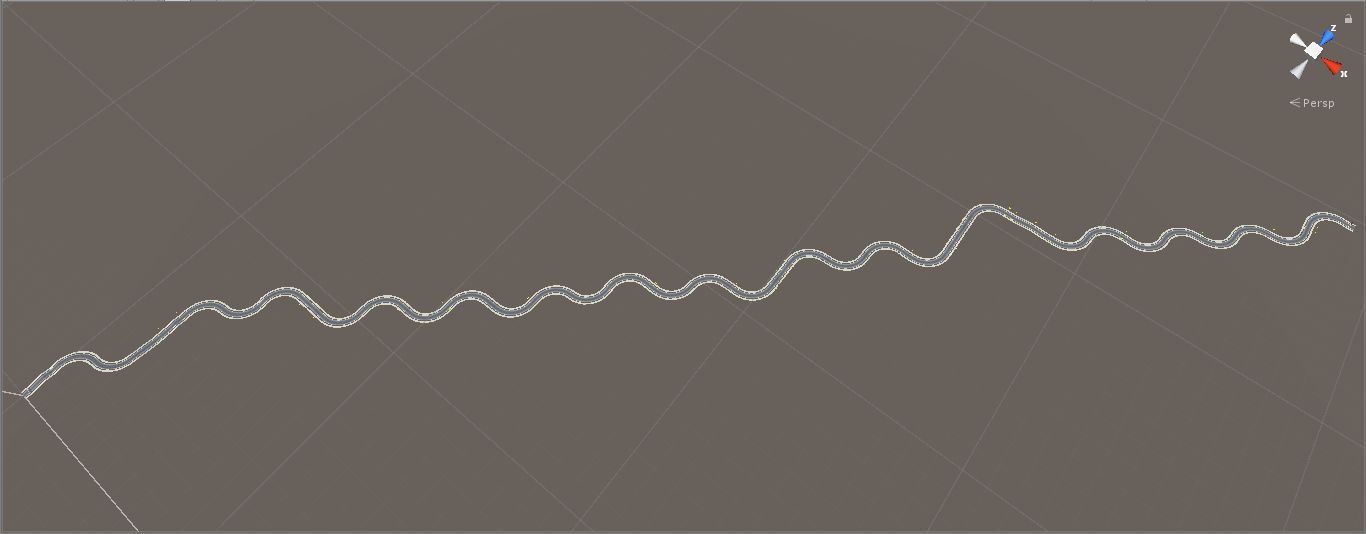
\includegraphics[width=1\columnwidth]{img/ProceduralTrack1.PNG}


\section{Scoreboard Screen}

Once the race is over, the host sends a list of player objects that includes their username and result to the scoreboard scripts, which then serializes them. It then passes them to the MariaDB as an XML list. The database then updates their records or creates a record if this is the players first game. This is then returned to the scoreboard and displayed to all the players.
\newline 

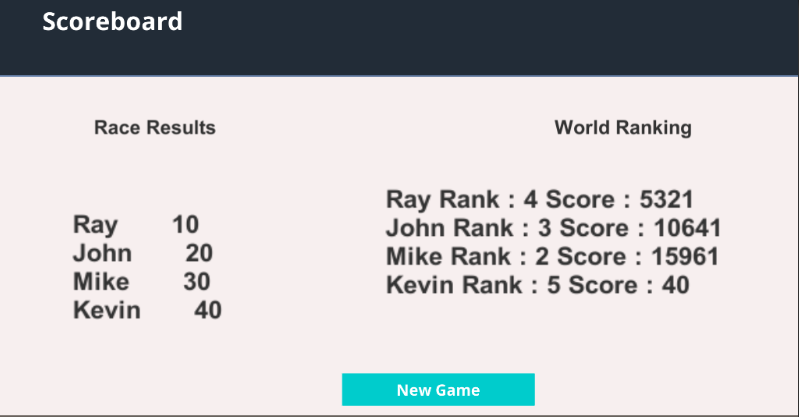
\includegraphics[width=1\columnwidth]{img/results.PNG}